%%%%%%%%%%%%%%%%%%%%%%%%%%%%%%%%
\section{Overview}
\label{sec:detectors-fd-alt-ov}

This chapter describes an alternative far detector design for
DUNE. The first detector module to be installed will use the reference
design, however this alternative design could be used for one or more
subsequent modules. This design implements a dual-phase liquid argon
time projection chamber (LArTPC) augmented with a light-readout
system. ``Dual-phase'' refers to the extraction of ionization
electrons at the interface between liquid and gas argon and their
amplification and collection in the gas phase.

The scope of the dual-phase far detector includes the design,
procurement, fabrication, testing, delivery, installation and
commissioning of the detector components:
\begin{itemize}
\item Charge-Readout Planes (CRP)
\item Field Cage and High-Voltage System  
\item Electronics, Chimney and Data Acquisition 
\item Slow Controls
\item Light-Readout System
\end{itemize}

The components and the liquid argon (LAr) will be housed in cryostats
provided by LBNF, described in \vollbnf.  As for the reference design
far detector, this alternative design satisfies the DUNE physics
requirements described in the reference design chapter.
Additional parameters specific to the dual-phase design are listed in
Table~\ref{tab:FD_req}.
\begin{cdrtable}[Dual-phase (alternative) far detector performance parameters]{llll}{FD_req}{Performance parameters specific to the dual-phase far detector design}  
Parameter & Requirement & Achieved Elsewhere & Expected Performance \\ \toprowrule
Gas phase gain & 20 & 200 & 20-100  \\ \colhline
Electron Lifetime & 3~ms &  $>3$~ms 35-t prototype  & $>5$~ms \\ \colhline 
Minimal S/N after 12 m drift & 9:1 &  $>100$:1 & 12:1-60:1  \\ 
\end{cdrtable}
This design incorporates some improvements with respect to the
reference design, namely a larger signal-to-noise ratio, a lower
detection threshold, a smaller pitch, a smaller number of readout
channels, two identical collection views, and the absence dead
materials in the LAr volume.  These advantages will be described in
this chapter, and are covered in detail in \anxlbnoa\ and \anxlbnob.


The alternative design is the outcome of 13 years of R\&D and of two
consecutive design study programs funded since 2008 by the European
Union: LAGUNA and LAGUNA-LBNO. The LAGUNA-LBNO design study was
concluded in August 2014.  In collaboration with industrial partners,
LAGUNA-LBNO designed an innovative, optimized and cost-effective
configuration for a long-baseline experiment.

The studies focused on the underground implementation of a very large
LAr detector (GLACIER) and involved many technical advances: such as
the tank, field cage and cathode, as well as logistics of the detector
assembly sequence and full costing. The full design and the related
technical developments are described in the documents submitted to the
EU at the conclusion of the design study, included with this CDR as
\anxlbnoa\ and \anxlbnob.

Following the GLACIER concept\cite{LAGUNA-LBNO-deliv} (see
Figure~\ref{fig:LBNO_50}), the dual-phase LArTPC detector design for
DUNE has a fully homogeneous liquid argon volume, where electrons
drift vertically towards the liquid-vapor interface. From there they
are extracted from the liquid into the gas phase, amplified and
collected on a segmented
anode\cite{Badertscher:2013wm,Badertscher:2012dq,Badertscher:2010zg}. 
\begin{cdrfigure}[The \ktadj{50} LBNO detector, GLACIER]{LBNO_50}{The \ktadj{50} LBNO detector, GLACIER}
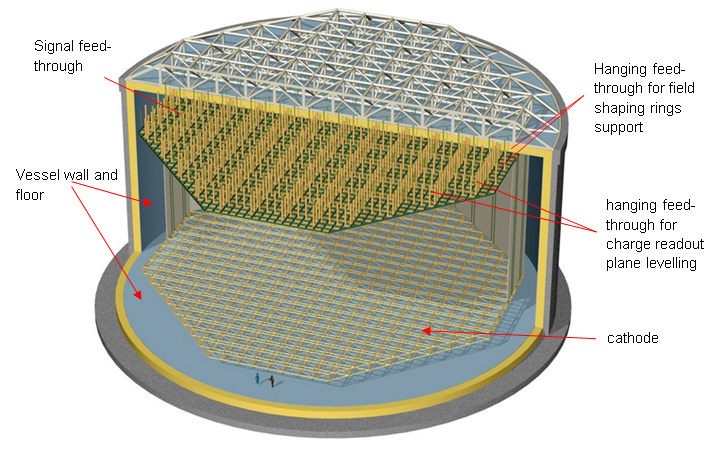
\includegraphics[width=0.9\linewidth]{LBNO50kton2}
\end{cdrfigure}
The electron amplification in the gas phase enables a robust and
tunable signal-to-noise ratio. Amplification of the ionization charge
in the extremely pure argon gas is achieved with micro-pattern
avalanche gas detectors called the Large Electron Multiplier
(LEM). The detector configuration is similar to a single-phase LArTPC
but with  unique features of the dual-phase design, e.g., high gain,
very long drift paths and large detector dimensions while minimizing
the number of readout channels.


An extraction efficiency of 100\% of the electrons from the liquid to
the gas phase is achieved with an electric field of the order of
2~kV/cm created by a submersed grid at the liquid-gas interface. The
ionization charge is then amplified by avalanches occurring in the gas
in the micro-pattern structure of the LEM and collected in a 2D
readout plane on the top of the gas volume. Readout units, combining
both the amplification and collection functions have an area of
0.5$\times$0.5~m$^2$ and are finely segmented with 3.125-mm-pitch
strips. The typical amplification achieved in this configuration is
around 20--100, which improves the S/N ratio and compensates for the
charge losses that occur due to the presence of electronegative
impurities along very long drift paths. Although the dual-phase TPC
has a longer drift length, it should be noted that it requires a LAr
purity similar to that for the single-phase TPC, around 0.1~ppb (or
100~ppt) of oxygen equivalent, corresponding to a 3~ms electron
lifetime.

This level of purity can be reached by starting from commercially
available ppm-level bulk argon and filling a non-evacuated
vessel\cite{WA105_TDR}.  The S/N ratio can exceed 100 for a minimum
ionizing particle (MIP) after a drift path of 12~m (assuming an
electron lifetime of 3~ms, a drift field of 0.5~kV/cm and a LEM gain
of 180). With the same drift field, electron-lifetime conditions and a
LEM gain of 25, the S/N is larger than 50:1 for tracks up to 6~m from
the anode; it reaches 14:1 for MIP tracks that are 12~m from the
anode.

The single drift field (E${\simeq}$0.5--1.0~kV/cm) inside the fully
active LAr volume is produced by applying high voltage to the cathode
plane at the bottom of the cryostat and is kept uniform by a stack
(field cage) of equally spaced field-shaping electrodes polarized at
linearly decreasing voltage from the cathode voltage to ground. Each
electrode is a rounded rectangle made of stainless-steel tubes
connected along a rectangular path with round corners.

The field cage is held in place by mechanical structures hung from the
top deck of the vessel that also provide insulation.  The cathode
structure is suspended from the field cage. The cathode plane is a
segmented structure of tubes of different sizes arranged in a grid in
order minimize its weight, limit sagging and avoid high electric field
regions in its proximity.  The grid allows scintillation light to pass
through and be detected by uniform arrays of photomultipliers mounted
at the bottom of the tank, 1~m below the cathode.

The drift field region is closed at the top by the anode, which
consists of an array of independent modules for the charge readout
called Charge Readout Planes (CRPs). Each CRP is composed of several
0.5$\times$0.5-m$^2$ readout units and is independently suspended
with stainless-steel ropes linked to the top deck. This suspension
system allows to adjust the CRP distance and parallelism with respect
to the LAr surface. The electrical signals from the collected charges
are then passed outside the tank via a set of dedicated signal
feedthrough chimney traversing the top layer of insulation. These
chimneys house at their bottom the cryogenic Front End (FE)
electronics.  The FE electronics are based on analog preamplifiers
implemented in CMOS ASIC circuits for high integration and large scale
affordable production. It is cooled at a temperature around 110 K and
is isolated with respect to the LAr vessel by a cold feedthrough. This
feedthrough is connected to the CRP via flat cables of 0.5~m
length. The chimneys design allows to access and replace the FE from
outside without contaminating the LAr volume. The digital electronics
and DAQ system are completely outside the cryostat and are housed in
micro-TCA racks mounted on each signal feedthrough chimney. Other
feedthrough chimneys are foreseen for the cathode HV connection, the
CRPs suspension and level adjustment, the high voltage and signal
readout of the PMTs and the monitoring instrumentation (level meters,
temperature probes, strain gauges, etc.)

Situated in the vapor phase on top of the LAr volume the CRP provides
an adjustable charge gain (with a minimal required gain of 20) and two
independent readout views, each with a pitch of 3.125~mm.  Combined
with the time information coming from the LAr scintillation readout by
the PMT arrays ($T_0$), the CRPs provide three-dimensional (3D) tracks
imaging with dE/dx information. The S/N ratio is increased by at least
one order of magnitude by the possibility of amplifying the charges
with avalanches in the gas phase.  This high S/N significantly
improves the event reconstruction quality. It also lowers the
threshold for small energy depositions and provides a better
resolution per volumetric pixel (voxel) compared to a single-phase
LArTPC.

The dual-phase TPC concept is well suited for large detector sizes
since the charge attenuation on long drift paths is compensated by the
charge amplification in the CRPs.  This configuration also simplifies
the construction by optimally exploiting long vertical dimensions of
the cryostat, reducing the number of readout channels, increasing the
detector size, and lowering costs.  This provides inside the TPC field
cage a large homogeneous fiducial volume for neutrino interactions,
consisting only of liquid argon with no embedded passive
materials. The charge produced in this volume is collected on the top
CRPs surface in a projective way, with practically no dead regions. In
each CRP the charge is readout in two collection views with no use of
induction views, which is also an important asset in the case of
complicated topologies.

The dual-phase readout scheme has been successfully demonstrated on
several prototypes through R\&D spanning more than 10 years.  The
design of very large (20--50~kt) underground detectors based on this
concept has been developed in great detail in the context of the
LAGUNA and LAGUNA-LBNO design studies.  The CERN WA105 experiment is
intended to show a full scale implementation of this technique, as
well as of other technologies developed for the construction of large
underground TPC detectors.  All the key subsystems of the WA105 LArTPC
demonstrator have been designed for scalability to larger detector
sizes.  This demonstrator will be tested and calibrated with a charged
particle beam (pion, muons, electrons) in 2018.


\section{Detector Configuration}

The proposed dual-phase detector module optimally exploits the
cryostat volume (14(w)$\times$14.1(h)$\times$62(l)~m$^3$) with an
anode active area of (12$\times$60~m$^2$) and a drift length of 12~m,
corresponding to an active mass of 12.096~kt of LAr (10.643~kt
fiducial). The design is based on the 20-kt LAGUNA-LBNO design study
with a CRP unit size adapted to the dimensions on the active area. The
cryostat height could be increased to achieve 15~m drift, resulting in
an active mass of 15.12~kt (13.444~kt fiducial).  This 15.1-kt
configuration, apart from the longer drift distance and field cage,
would have the same characteristics of the 12.1-kt configuration,
given that the covered active area is exactly the same. With these
transverse dimensions every additional meter of drift length provides
a 1-kt increase in the active mass at a moderate additional cost.

The inner detector for the 12.1-kt active mass is built as a single
active volume 60~m long, 12~m wide and 12~m high. The active volume
(see Figures~\ref{fig:DP_det1} and~\ref{fig:DP_det2}) is surrounded by
a vertical field cage made up of 60 rectangular tubular rings (tubes
diameter 140~mm, rings vertical pitch 200~mm).
\begin{cdrfigure}[Dual-phase detector 3D view]{DP_det1}{The DUNE dual-phase 
detector with cathode, PMTs, field cage and anode plane with chimneys.}
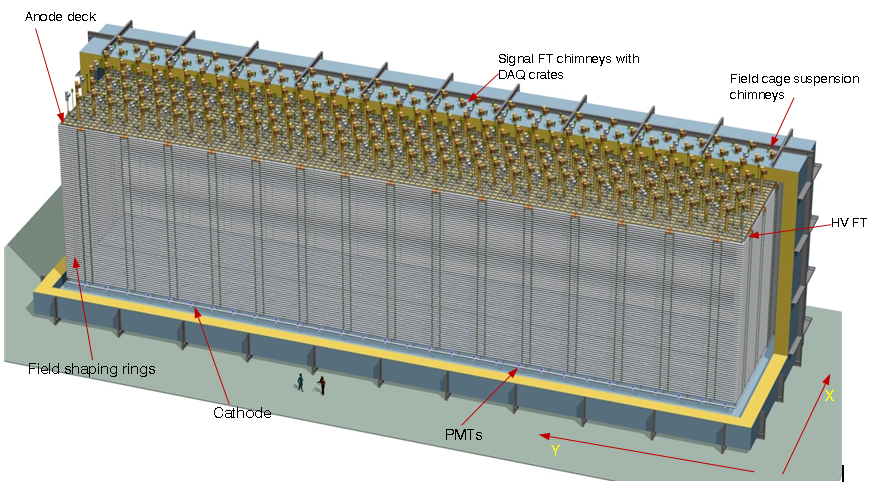
\includegraphics[width=\linewidth]{DUNE12_FC}
\end{cdrfigure}
\begin{cdrfigure}[Dual-phase detector 3D view (partially open)]{DP_det2}
{The DUNE dual-phase detector (partially open) with cathode, PMTs, field cage and anode plane with chimneys.}
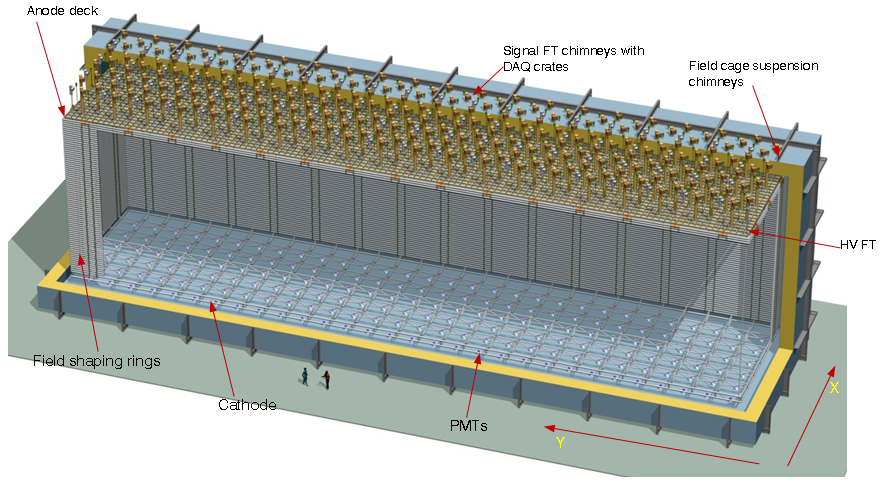
\includegraphics[width=\linewidth]{DUNE12_open}
\end{cdrfigure}

The cathode plane (on the bottom) is made by a reinforced frame, to
guarantee its planarity, filled by a tubular grid (not visible in
Figure~\ref{fig:DP_det2}) to allow the optical transparency for the
scintillation light towards an array of 180 PMTs (1 per 4~m$^2$)
located at the bottom of the vessel.

The ionization electrons in the liquid phase drift towards the CRPs
(Charge Readout Planes) in a uniform electric field. The extraction of
the electrons from the liquid to vapor phase is performed thanks to a
submersed horizontal extraction grid, integrated in the CRP structure.
Each CRP is composed of LEM/Anode Sandwiches (LAS)
(0.5~m$\times$0.5~m) embedded in a mechanically reinforced frame of
FR-4 and Stainles Steel.  Each sandwich includes a LEM (Large Electron
Multiplier) for the charge amplification via avalanches occurring in a
micro-pattern structure in pure gas argon and an anode Printed Circuit
Board (PCB) for the collection of the amplified charges on two
independent orthogonal views with interleaved X and Y strips.
Thicknesses and possible biasing voltages for the different layers are
indicated, as example, in Figure~\ref{fig:CRP_struct}.
\begin{cdrfigure}[Charge Readout Plane (CRP) structure]{CRP_struct}
{Thicknesses and HV values for e- extraction from liquid to gaseous Ar, their 
multiplication by LEMs and their collection on the X-Y CRP plane. The 
HV values are indicated for a drift field of 0.5~kV/cm in LAr.}
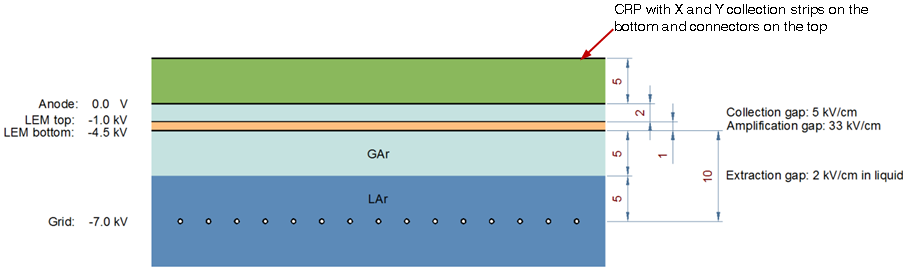
\includegraphics[width=\linewidth]{CRP_gaps.png}
\end{cdrfigure}

The anode plane, at the top of the active volume, is made by an array
of 45 independent CRP modules, 3$\times$3~m$^2$ each, as shown in
Figure~\ref{fig:CRP_unit1} and Figure~\ref{fig:CRP_unit2} Each CRP
unit includes 36 (0.5~m$\times$0.5~m) LAS.
\begin{cdrfigure}[DUNE CRP 3~m$\times$3~m units.]{CRP_unit1} {Two DUNE CRP 3~m$\times$3~m units side by side. On the left one of the 79 equal 
CRP units, on the right the 1$^{st}$ CRP unit with a chamfered LEM/Anode Sandwich  for the insertion of the high voltage feedthrough.}
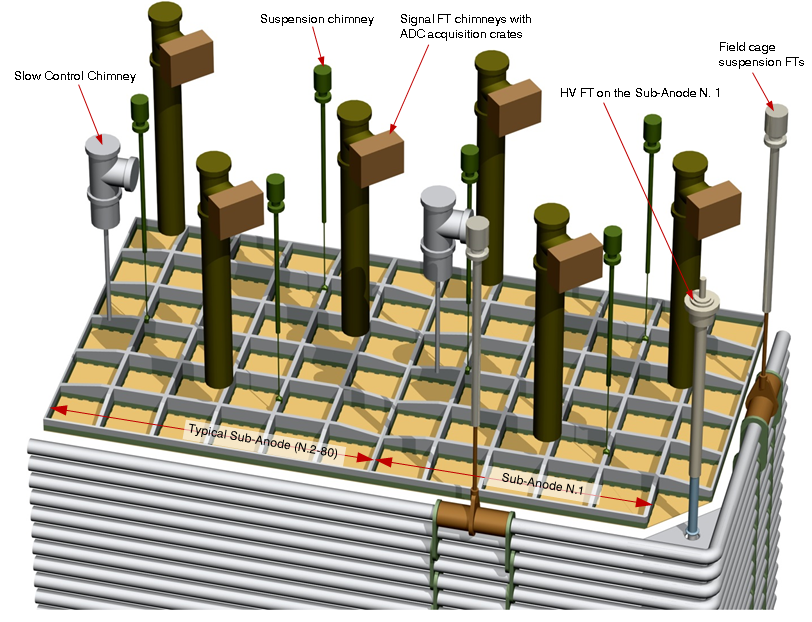
\includegraphics[width=.7\linewidth]{DUNE12_units}
\end{cdrfigure}
\begin{cdrfigure}[Signal collection in the X and Y views by the 3 SFT chimneys.]
{CRP_unit2}{Signal collection in the X and Y views of the  3$\times$3~m$^2$ DUNE CRP unit by the 3 SFT chimneys.}
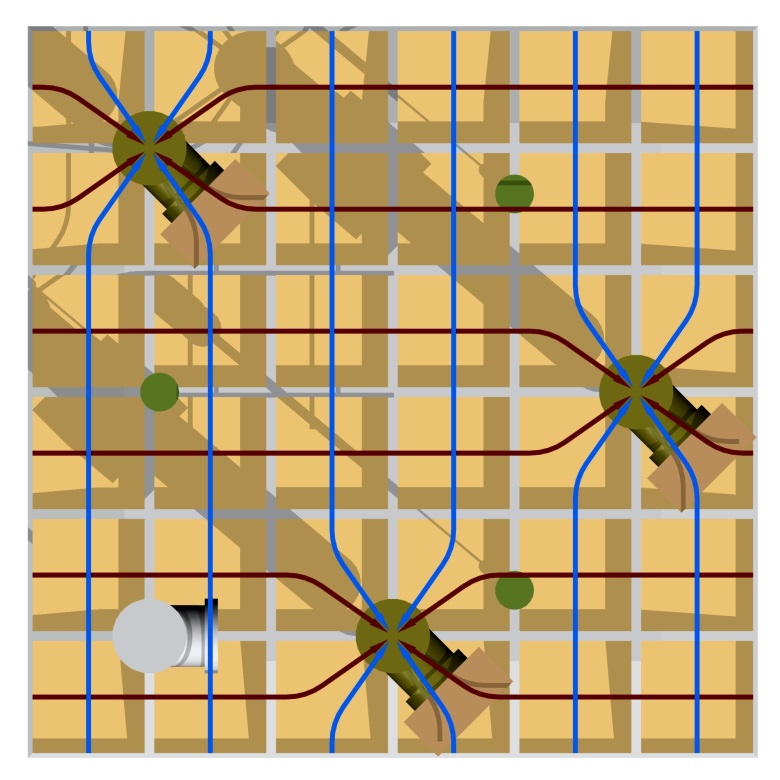
\includegraphics[width=.5\linewidth]{DUNE12_CRP}
\end{cdrfigure}

Signals in each CRP unit are collected via 3 signal feedthrough
chimneys. Each chimney collects 640 readout channels and hosts at its
bottom the front-end cards with the cryogenic electronics (ASIC
amplifiers), just before a cold feedthrough isolating them from the
ultra-pure LAr volume. The front-end cards work at a temperature of
110 K and can be removed from the top of the chimney without
contaminating the LAr volume. The LEM/Anode sandwiches in the same CRP
unit are interconnected with short flat cables so that each readout
channel corresponds to a total strips length of 3~m.
  
Each CRP unit is independently suspended by 3 stainless steel
ropes. The vertical level of each CRP unit can then be automatically
adjusted with respect to the LAr level via 3 suspension feedthroughs,
electrically operated from outside. A Slow Control feedthrough +
chimney, one per CRP unit, is used for the signals readout for level
meters and the temperature probes and to apply the HV bias on the two
sides of the LEMs and on the extraction grid.

The extraction grid integrated in the CRP is made by an array of X and
Y oriented stainless steel wires, 0.1~mm in diameter with 3.125~mm
pitch.  Wires, $\sim$3~m long in X and $\sim$3~m long in Y directions,
have their sags minimized to $\sim$0.1~mm thanks to X and Y oriented
supporting combs blades (see Figure~\ref{fig:Wires_comb}) inserted
between anode planes of 1~m$\times$1~m size. The array of blades
penetrates the liquid close to the surface and have the additional
benefit of maintaining the liquid level flat.
\begin{cdrfigure}[Wires hanging comb blade.]{Wires_comb}{Wires hanging comb blade.}
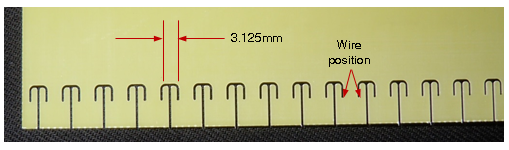
\includegraphics[width=.6\linewidth]{Wires_comb.png}
\end{cdrfigure}


The number of components and parameters for the 12~kt (15~kt)
dual-phase LArTPC are summarized in Tables~\ref{tab:DP_params}
and~\ref{tab:DP_numbers}.
\begin{cdrtable}[Sizes and Dimensions for the 12~kt (15~kt) dual-phase LArTPC]{lll}
{DP_params}{Sizes and Dimensions for the 12~kt (15~kt) dual-phase  LArTPC}  Item & Value(s) &  \\ \toprowrule
Active volume width and length & W = 12~m &  L = 60~m \\ \colhline
Active volume height &  H = 12~m (H = 15~m)  &  \\ \colhline
Active volume/LAr mass & 8,640 (10,800)~m$^3$ &  12,096 (15,120) metric ton \\ \colhline
Field ring vertical spacing & 200~mm  \\ \colhline
Field ring tube diameter & 140~mm \\ \colhline
Anode plane size & W = 12~m & L = 60~m \\ \colhline
CRP unit size & W = 3~m & L = 3~m  \\ \colhline
HV for vertical drift & 600--900~kV \\ \colhline
Resistor value & 100~M$\Omega$ \\ 
\end{cdrtable}
\begin{cdrtable}[Quantities of Items for the 12~kt (15~kt) dual-phase LArTPC]{ll}{DP_numbers}{Quantities of Items for the 12~kt (15~kt) dual-phase  LArTPC}  Item & Number    \\ \toprowrule
Field rings & 60  (75)  \\ \colhline
CRP units & 4 $\times$ 20 = 80 \\ \colhline
LEM/Anode sadwiches per CRP unit & 36 \\ \colhline
LEM/Anode sandwiches (total) & 2,880 \\ \colhline
SFT chimneys / CRP unit & 3 \\ \colhline
SFT chimneys (total) & 240 \\ \colhline
Readout channels / SFT chimney & 640  \\ \colhline
Readout channels (total) & 153,600 \\ \colhline
Suspension FT / CRP unit & 3  \\ \colhline
Suspension FTs (total) & 240  \\ \colhline
Slow Control FT / sub-anode & 1  \\ \colhline
Slow Control FTs (total) & 80 \\ \colhline
HV feedthrough & 1  \\ \colhline
Voltage degrader resistive chains & 4 \\ \colhline
Resistors (total) & 240 (300)  \\ \colhline
PMTs (total) & 180 (1/4~m$^2$) \\ 
\end{cdrtable}
